% Manual of pgf-umlcd.sty, a convenient set of macros for drawing UML
% class diagrams.
% Written by Xu Yuan <xuyuan.cn@gmail.com>
% This file is part of pgf-umlcd
% you may get it at http://code.google.com/p/pgf-umlcd/

\documentclass{article}
\usepackage[margin=12mm]{geometry}
\usepackage{hyperref}

\usepackage[
% school,
% simplified
]{pgf-umlcd}

%%%%%%%%%%%%%%%%%%%%%%%%%%%%%%%%%%%%%%%%%%%%%%%%%%%%%%%%%%%%%%%%%
\usepackage{listings}
\usepackage{color}
\definecolor{listinggray}{gray}{0.92}
\lstset{ %
language=[LaTeX]TeX,
breaklines=true,
frame=single,
% frameround=tttt,
basicstyle=\footnotesize\ttfamily,
backgroundcolor=\color{listinggray},
keywordstyle=\color{blue}
}
%%%%%%%%%%%%%%%%%%%%%%%%%%%%%%%%%%%%%%%%%%%%%%%%%%%%%%%%%%%%%%%%%

%%%%%%%%%%%%%%%%%%%%%%%%%%%%%%%%%%%%%%%%%%%%%%%%%%%%%%%%%%%%%%%%%
\hypersetup{
  colorlinks=true,
  linkcolor=blue,
  anchorcolor=black,
  citecolor=olive,
  filecolor=magenta,
  menucolor=red,
  urlcolor=blue
}
%%%%%%%%%%%%%%%%%%%%%%%%%%%%%%%%%%%%%%%%%%%%%%%%%%%%%%%%%%%%%%%%%

%%%%%%%%%%%%%%%%%%%%%%%%%%%%%%%%%%%%%%%%%%%%%%%%%%%%%%%%%%%%%%%%%
\newcommand{\demo}[2][1]{
\begin{minipage}{.49\linewidth}
\centering
\resizebox{#1\linewidth}{!}{
\input{demo/#2}
}
\end{minipage}
\hspace{0.01\linewidth}
\begin{minipage}{.5\linewidth}
\lstinputlisting{demo/#2}
\end{minipage}
}
%%%%%%%%%%%%%%%%%%%%%%%%%%%%%%%%%%%%%%%%%%%%%%%%%%%%%%%%%%%%%%%%%

%%%%%%%%%%%%%%%%%%%%%%%%%%%%%%%%%%%%%%%%%%%%%%%%%%%%%%%%%%%%%%%%%
\newcommand{\example}[1]{
\resizebox{\linewidth}{!}{
\input{demo/#1}
}
\lstinputlisting{demo/#1}
}
%%%%%%%%%%%%%%%%%%%%%%%%%%%%%%%%%%%%%%%%%%%%%%%%%%%%%%%%%%%%%%%%% 

\begin{document}
%%%%%%%%%%%%%%%%%%%%%%%%%%%%%%%%%%%%%%%%%%%%%%%%%%%%%%%%%%%%%%%%%
\title{Drawing UML Class Diagram by using \texttt{pgf-umlcd}}
\author{\href{mailto:xuyuan.cn@gmail.com}{Yuan Xu}}
\date{\today{}~(v0.2.1)}
\maketitle
%%%%%%%%%%%%%%%%%%%%%%%%%%%%%%%%%%%%%%%%%%%%%%%%%%%%%%%%%%%%%%%%%

\begin{abstract}
  \texttt{pgf-umlcd} is a LaTeX package for drawing UML Class
  Diagrams. As stated by its name, it is based on a very popular
  graphic package \texttt{PGF/TikZ}. This document presents the usage
  of \texttt{pgf-umlcd} and collects some UML class diagrams as
  examples. \texttt{pgf-umlcd} can be downloaded from
  \href{http://code.google.com/p/pgf-umlcd/}{http://code.google.com/p/pgf-umlcd/}.
\end{abstract}

\tableofcontents

\section{Basics}
\subsection{Class with attributes and operations}
Note: If you don't want to show empty parts in the diagrams, please
use \texttt{simplified} option, e.g. \lstinline|\usepackage[simplified]{pgf-umlcd}|.\\
\demo{class}



\section{Mon TEST }

\subsection{Le diagramme de classe }
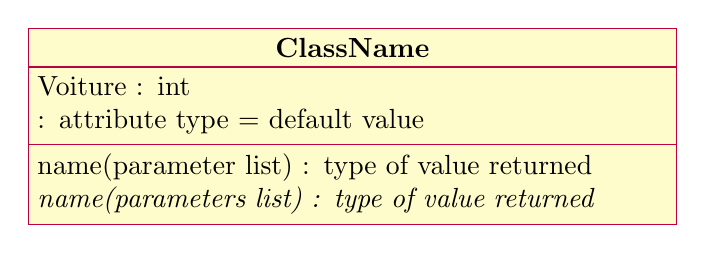
\begin{tikzpicture}
  \begin{class}[text width=8cm]{ClassName}{0,0}
    \attribute{Voiture : int}
    \attribute{ : attribute type = default value}

    \operation{name(parameter list) : type of value returned}
    % virtual operation
    \operation[0]{name(parameters list) : type of value returned}
  \end{class}
\end{tikzpicture}


\end{document}
%%% Local Variables: 
%%% mode: Tex-PDF
%%% TeX-master: t
%%% End: 
